%##############################################################################
% Preamble
%##############################################################################

\documentclass{pset}
\name{Dustin Tran, Xiaomin Wang, Rodrigo Gomes}
\email{\{trandv,xiaominw, rgomes\}@mit.edu}

\course{6.834J/16.412J, S15}
\instructor{Professor Brian Williams}
\assignment{Problem Set \#3}
\duedate{April 17, 2015}

\begin{document}

%##############################################################################
% Begin Document
%##############################################################################

\section{Introduction}
Many scenarios in real life occur where one must make a sequence of decisions
under uncertainty. Quite often in these scenarios two unknowns exist: the
result of taking an action at a given state and the true state of the agent at
any point in time. This is similar to that of a hidden Markov model (HMM), only
in that one must make a sequence of actions instead of a single action; thus the
problem falls no longer in supervised learning but reinforcement learning. The
classic example is a robot which tries to navigate a discrete environment using a
GPS, and it performs action that lead to different states with various
probabilities. The transition probabilities are unknown, and because of the GPS,
there is also inaccuracy in what the
underlying state is.

One can formalize the problem, under Markovian assumptions, as a partially
observable Markov decision process (POMDP). In this project we provide a
software library for implementing and solving them, which is modular and
flexible enough for further development and user-specified agents/environments.
We encode a variety of basic tasks and solve them using a combination of value
iteration and several standard (PO)MDP solvers---one is a variant of Thompson
sampling \cite{strens2000bayesian}, which is a Bayesian approach following a
Dirichlet-multinomial posterior over each state-action pair.

The repository can be found at https://github.com/dustinvtran/bayesrl.
To install from pip, run
\begin{lstlisting}
pip install -e "git+https://github.com/dustinvtran/bayesrl.git#egg=bayesrl"
\end{lstlisting}

\section{Technical Background}

\subsection{POMDP}
POMDP is a generalization of a Markov decision process (MDP). In a MDP, for each
possible state of the process, a decision has to be made regarding which action
should be executed in that state. The chosen action and given state affects the
costs (or rewards) incurred. The goal is to learn the optimal \emph{policy},
which is a
choice of actions that in expectation leads to the optima reward in a
pre-defined number of steps (in the case of finite horizon; or in infinite time). In a
POMDP model, the agent does not fully observe the underlying states but a
(non-sufficient) statistic of it. Thus POMDPs also
maintain a probability distribution over the set of possible states, based on a
set of observations and observation probabilities, and the underlying MDP.

More formally, a POMDP is a collection $(S,A,T,R,\Omega,O,\gamma)$, where

\begin{itemize}
\item $S$ is a set of states
\item $A$ is a set of actions
\item $T$ is a set of transition probabilities between states. If the agent is currently in state $s
\in S$, and it takes action $a \in A$, the agent will transition to a new state
$s'$ with probability
$T(s' \mid s,a)$.
\item $R: S \times A \rightarrow \mathbb{R}$ is a reward function that assigns a numeric reward (or
cost if the value is negative) for each state and action.
\item $\Omega$ is a set of observations
\item $O$ is a set of conditional observation probabilites. If the agent is now in state $s$,
it receives an observation $o$ according to $O(o \mid s)$
\item $\gamma \in [0,1]$ is a discount factor that determines how much rewards should be discounted over time
\end{itemize}

We use our testing environment \texttt{GridWorld} as an example.
\texttt{GridWorld} represents a 2D maze where the agent can be in discrete locations.
Certain locations are impossible for the agent to move to, representing ``walls''. Every
action can move the agent between two adjacent grid locations, or fail, and
cause
the agent to take a uniformly random action instead according to some
user-specified probability. The goal is to reach
the goal location in least amount of time, as each move is -1 reward, hitting a
wall is -1 reward, and reaching the end positions incurs a reward of +50.

For \texttt{GridWorld}, $S$ consists of all the possible (row, column) location
tuples inside the maze.  $A$ contains the four possible actions the agent can
take: up, down, left, right.  $T$ describes a transition model that allows the
agent to move without hitting the wall.  We define $R$ as the above. To make
this a partially observable problem, we implemented two observation models.
\begin{itemize}
\item
The
easier model gives the agent more information about the environment. The agent
knows which of its four neighbors are walls, giving rise to 16 total
observations.
\item
In the second observation model, the agent can only observe how
many of its four neighbors are walls, giving rise to 5 possible observations.
$O$ is such that $Pr(true\_observation\mid state)=true\_observation\_prob$,
where $true\_observation\_prob$ can be adjusted, and
\begin{equation}
Pr(other\_observation\mid
state)=\frac{1-true\_observation\_prob}{total\_num\_of\_observations-1}
\end{equation}
\end{itemize}
Since
we cannot work with the underlying states directly in POMDP, we also need $B$
which is the set of belief states, or the probabilities the agent is at all
possible states.

\subsection{Thompson Sampling}
Thompson Sampling is used to learn the transition distribution $T$, where one
first specifies a prior according to one's knowledge about the transitions
before trying any actions. After a constant set of time steps, the transition
probabilities are then recalculated using a posterior update following a
Dirichlet-multinomial distribution. In MDP, since the agent observes the states
directly, the posterior transition probabilities are updated directly using the
transition counts. In POMDP, the posterior probabilities are iteratively updated
following an update on belief state transition probabilities.

Note that we've also implemented a variety of other standard MDP solvers for
benchmarking: Q-Learning, SARSA, and R-MAX.

\subsection{Value Iteration}
Given estimated transition probabilities, we then solve for the underlying policy with value iteration. Value $V$, is the expected total reward
given a policy $\pi$, where a policy decides which action to take given the
belief state. $a = \pi(b)$. The expected reward for policy $\pi$ starting freom
belief $b_0$ is defined as
\[ V^{\pi}(b_{0})=\sum\limits_{t=0}^\infty \gamma^{t}r(b_t,a_t) \]
where $r(b_t, a_t) = \sum\limits_{s \in S} b_t(s)R(s,a_t)$.
The optimal policy should maximize the long term reward
\[ \pi = \underset{\pi}{\text{argmax}} V^{\pi}(b_0) \]
At each time step, we update the belief states based on the observation, and
then update the values based on the updated belief states. The action that gives
the largest expected reward over the belief states is selected for the next time
step. The values gradually improve until convergence.
By improving the values, the policy is implicitly improved.

\section{Implementation}

\subsection{Agent Environment Paradigm}
For MDP, we follow the paradigm set forth in Sutton and Barto (Figure 3.1,
\cite{sutton1998reinforcement}).
\begin{figure}[ht]
\begin{center}
\centerline{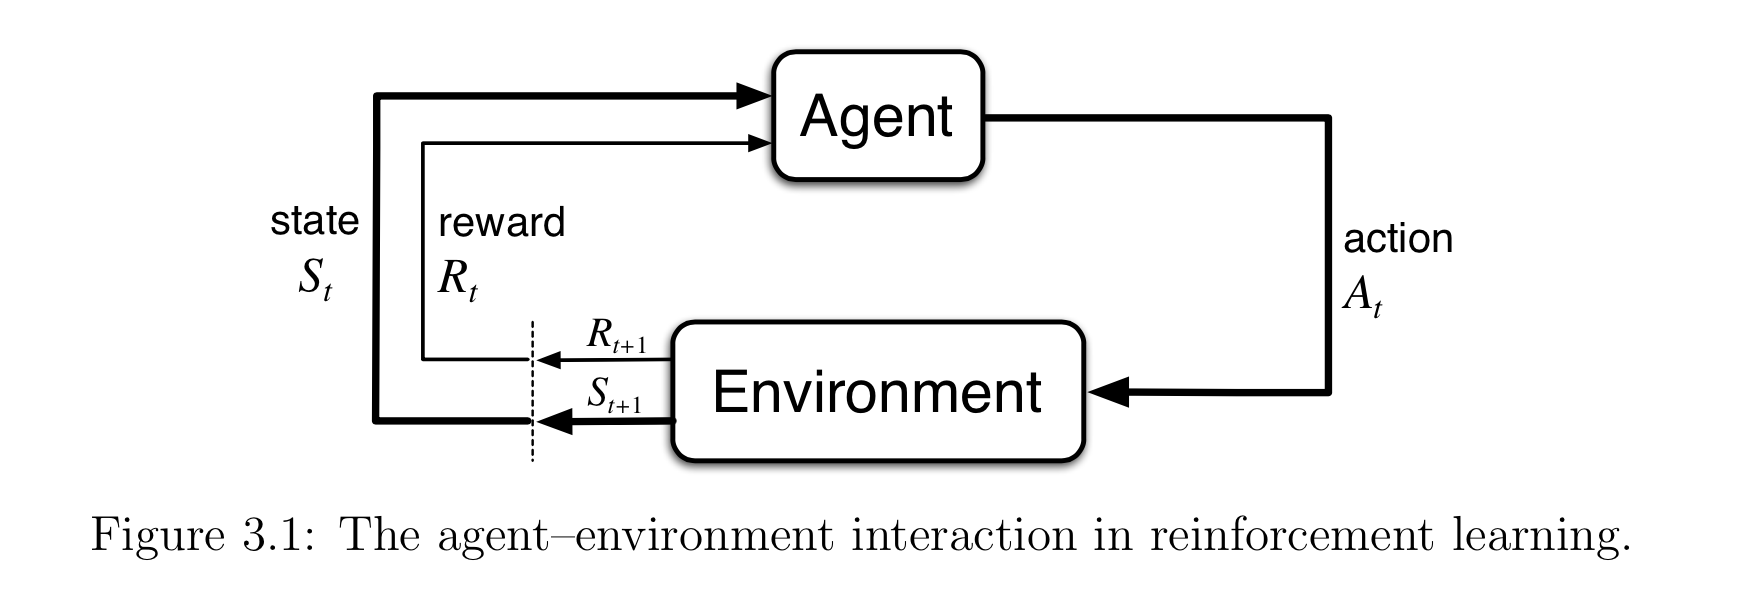
\includegraphics[width=\textwidth]{img/agent_environment.png}}
\end{center}
\end{figure}
It suggests that RL agents need only output a suggested action after previous history and a given state and reward.  Overall by following the paradigm for the software design, we make the learning process explicit and intuitive.

\subsubsection{Agent}
We implement a base class \texttt{Agent} which is a collection of objects and functions to be used for all other agents. Agents differ primarily in their \texttt{interact()} function, which determines the next action to perform given a state and reward from the environment.

The model-based algorithms R-MAX and Thompson sampling inherit from \texttt{ModelBasedAgent}, which is a class that itself inherits from \texttt{Agent}; \texttt{ModelBasedAgent} adds subroutines specific to model-based approaches such as value iteration.

In order to reduce the most redundant code, we also could have used an
additional class that inherits from \texttt{Agent} for temporal difference method agents; this
would be used by both \texttt{SARSAAgent} and \texttt{QLearningAgent}, as they
differ only in their \texttt{value\_table} assignment. However, the efficiency gain in such an
abstraction is not worth the loss of readability in our opinion.

\subsubsection{Environment}
An \texttt{Environment} object is initialized at some state, with an arbitrarily
defined state and action space. Actions are performed on an \texttt{Environment}
object under the subroutine \texttt{perform\_action()}, and the output is a new state and its reward.

\subsubsection{Trial and Plot}
As for trials, we implement a class \texttt{Trial} which contains all information for running multiple trials, i.e., independent collections of episodes to learn and act upon. We also add a \texttt{Plot} class which is a wrapper containing all \texttt{Trial} objects; this is convenient for generating plots on collections of trials coming from possibly many different agents.

\subsection{POMDP}
For POMDP, we assume that the agent is given an observation model of the
environment it is acting in, in the form of a conditional probability distribution
$P(observation \mid state)$. Astr\"{o}m has shown that a properly updated probability
distribution over the state space $S$ is sufficient to summarize all the observable
history of a POMDP agent without loss of optimality \cite{astrom1965optimal}. 
Thus we add a step of updating the belief state to the MDP paradigm. And the belief state, instead
of the underlying state, is used to update the transition model.

\subsection{Organization of Code}
We follow the directory structure specified in the problem set, with two
exceptions:
\begin{itemize}
\item \texttt{documentation/} does not exist. Instead, documentation is written
in the \texttt{README.md} inside the current working directory. Any additional
documentation not purely necessary for the problem set submission is in the
Github wiki (which is a subset of anything in this writeup).
\item \texttt{source/} is named \texttt{bayesrl/} in order to follow Python
convention for installing modules.
\end{itemize}

\section{Analysis}

\subsection{Runtime}
The algorithm takes $O(\mid S \mid ^2 \mid A \mid)$ to calculate the transition probabilities, the
expected rewards and the belief state. It is uncertain how many time steps are required for
convergence. All solvers we implement are guaranteed to converge in polynomial time for MDPs,
although unfortunately we have not seen stricter theoretical results on the
upper bounds than this. This certainly makes sense as it is true for all
environments regardless of the pathological scenario. However, it would
certainly be interesting to examine bounds under stricter assumptions where we
fix the environment and perhaps certain parameter settings to simplify the
analysis.

\subsection{Memory}
We to store several arrays for the computation. The transition probabilities
table is of dimension $\mid S \mid ^2 \mid A \mid$. The value table is of
dimension $\mid S \mid \mid A \mid$. The transition observation table is of
dimension $\mid S \mid ^2 \mid A \mid$. Thus the space requirement for the
algorithm is $O(\mid S \mid ^2 \mid A \mid)$.

\subsection{Limitations}
If the number of states is large, the algorithm quickly becomes intractable. We
are quite interested in examining function approximations, which allow one to
essentially apply a supervised learning algorithm to predict the optimal action
given state characteristics, rather than to hardcode them manually. Note
however that this makes the runtime even worse as there is an additional error
accumulating as a result of the predictions.

\section{Experiments}
The implementation of Thompson Sampling for MDPs ran very successfully: as time
progressed, the agent was able to get to the goal much faster, and get a high
reward. It did not work, however, for POMDPs. As time progressed, the agent seemed
to take about the same amount of time to reach the goal on every execution, not
improving in performance. We hypothesize that the reason is due to a lack of
a good prior on the transition model: Thompson sampling relies a lot on being
able to count the number of transitions between states, given an action.

\begin{figure}[ht]
\begin{center}
\centerline{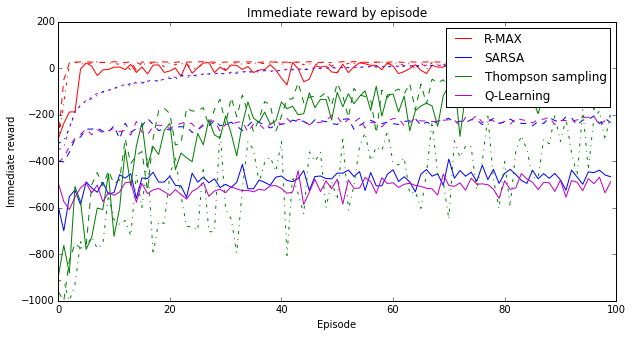
\includegraphics[width=\textwidth]{img/mdp_imm_rewards.png}}
\caption{Immediate reward for MDP solvers in a variety of parameter settings on
the Gridworld example.
Each of the settings for Thompson sampling vary how strong the misspecification of the
prior as a uniform distribution, and yet in all three scenarios it indicates
convergence. We also see that R-MAX performs better than the temporal difference methods.}
\end{center}
\end{figure}

This is very hard in a POMDP with a weak prior on its transition model, as it
may have a completely wrong idea of where it ends up at each step. The
observation model is supposed to improve its accuracy, but it was not sufficient
in this case. In fact, we can see this empirically by essentially hardcoding the
optimal path by putting high probability on where it should go, and indeed it
converges to the optimal quite quickly.

To have an idea of how differently successful the same approach was on MDPs vs
POMDPs, we show you our results:

\begin{figure}[ht]
\centering
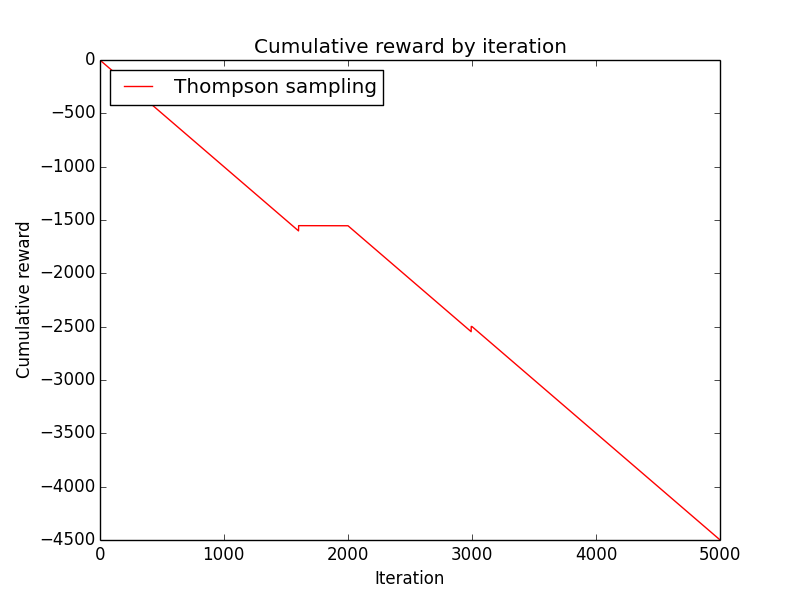
\includegraphics[width=0.75\textwidth]{img/pomdp.png}
\caption{\label{fig:pomdp}Cumulative Reward for POMDP}
\end{figure}

These graphs show the cumulative reward that the agent got as time progressed.
In the MDP case, the reward started low, and kept getting lower, as the agent
explored. It, however, started getting higher as the agent started acting in a
more deliberate manner, to maximize reward. The POMDP agent, however, seems to
be in a state where its reward just gets increasingly negative. It is unclear
whether it never leaves the exploration phase, or if it simply learns a completely
wrong transition model, and thus computes a very wrong policy.

\bibliography{6_834j_ps03}
\bibliographystyle{plain}

%##############################################################################
% End Document
%##############################################################################

\end{document}
